\documentclass[twoside,11pt]{starlink}

% ? Specify used packages
% ? End of specify used packages

% -----------------------------------------------------------------------------
% ? Document identification
% Fixed part
\stardoccategory    {Starlink Cookbook}
\stardocinitials    {SC}
\stardocsource      {sc\stardocnumber}
\stardoccopyright
{Copyright \copyright\ 1997 Council for the Central Laboratory of the Research C
ouncils}
\stardocnumber      {9.1}
\stardocauthors   {M D Lawden\\
                                Anne Charles}
\stardocdate        {14 May 1997}
\stardoctitle       {\LaTeX\ Cookbook}
\stardocabstract  {This cookbook shows some examples of
\LaTeX\ in action and should help you to
get to know how to use \LaTeX\ effectively.}
% ? End of document identification
% -----------------------------------------------------------------------------
% ? Document specific \providecommand or \newenvironment commands.
\providecommand{\radec}{$[\alpha,\delta\,]$}
\providecommand{\mhadec}{$[-h,\delta\,]$}
\providecommand{\azel}{$[A,E\,]$}
% ? End of document specific commands
% -----------------------------------------------------------------------------
%  Title Page.
%  ===========
\begin{document}
\scfrontmatter


\section{Introduction\xlabel{introduction}}

This paper shows some examples of \LaTeX\ in action and should help you to
get to know how to use \LaTeX\ effectively.
Sample inputs to \LaTeX\ are shown on the left hand pages and the output they
generate when processed by \LaTeX\ is shown on the opposite page.
When starting to prepare a \LaTeX\ document, copy a skeleton such as
/star/docs/sun.tex and edit as required.

These examples are just to enable you to get going quickly with \LaTeX\
and are not meant to be exhaustive.
Also, I do not claim that these techniques are the best possible; only that
they work.
For serious users, there is no substitute for Leslie Lamport's book
``\LaTeX\ User's Guide \& Reference Manual".
Copies of this book may be available for loan; ask your Site Manager.
You should also read \xref{SUN/9}{sun9}{} before attempting to use \LaTeX.

The methods shown in this paper were stolen from many sources.
If you see a format in a Starlink paper that you like, you can always look
in the document source in /star/docs to see how it was done.

\newpage

\section {Document structure\xlabel{document_structure}}

\begin{terminalv}
\section  {Introduction}
     <text>
\section{The Starlink Project}
     <text>
\subsection{Operation and Management}
     <text>
\section{Users}
     <text>
\section{Finding information}
     <text>
\subsection{VAX Documents}
     <text>
\subsection{Starlink Documents}
     <text>
\subsection{On-line Files}
     <text>
\subsubsection{Starlink documents}
     <text>
\subsubsection{Information summaries}
     <text>
\paragraph {Starlink-wide information}
     <text>
\paragraph {Local information}
     <text>
\subsubsection{Internal documents}
     <text>
\subsubsection{Hints}
     <text>
\section{Hardware}
     <text>
\section{Software}
     <text>
\appendix
\section{Personnel}
     <text>
\section{Inventory}
     <text>
\end{terminalv}

\newpage

\begin{center}
  \textbf{\LaTeX\ OUTPUT}
% Paste sc9a in here
  \begin{figure}[h]
    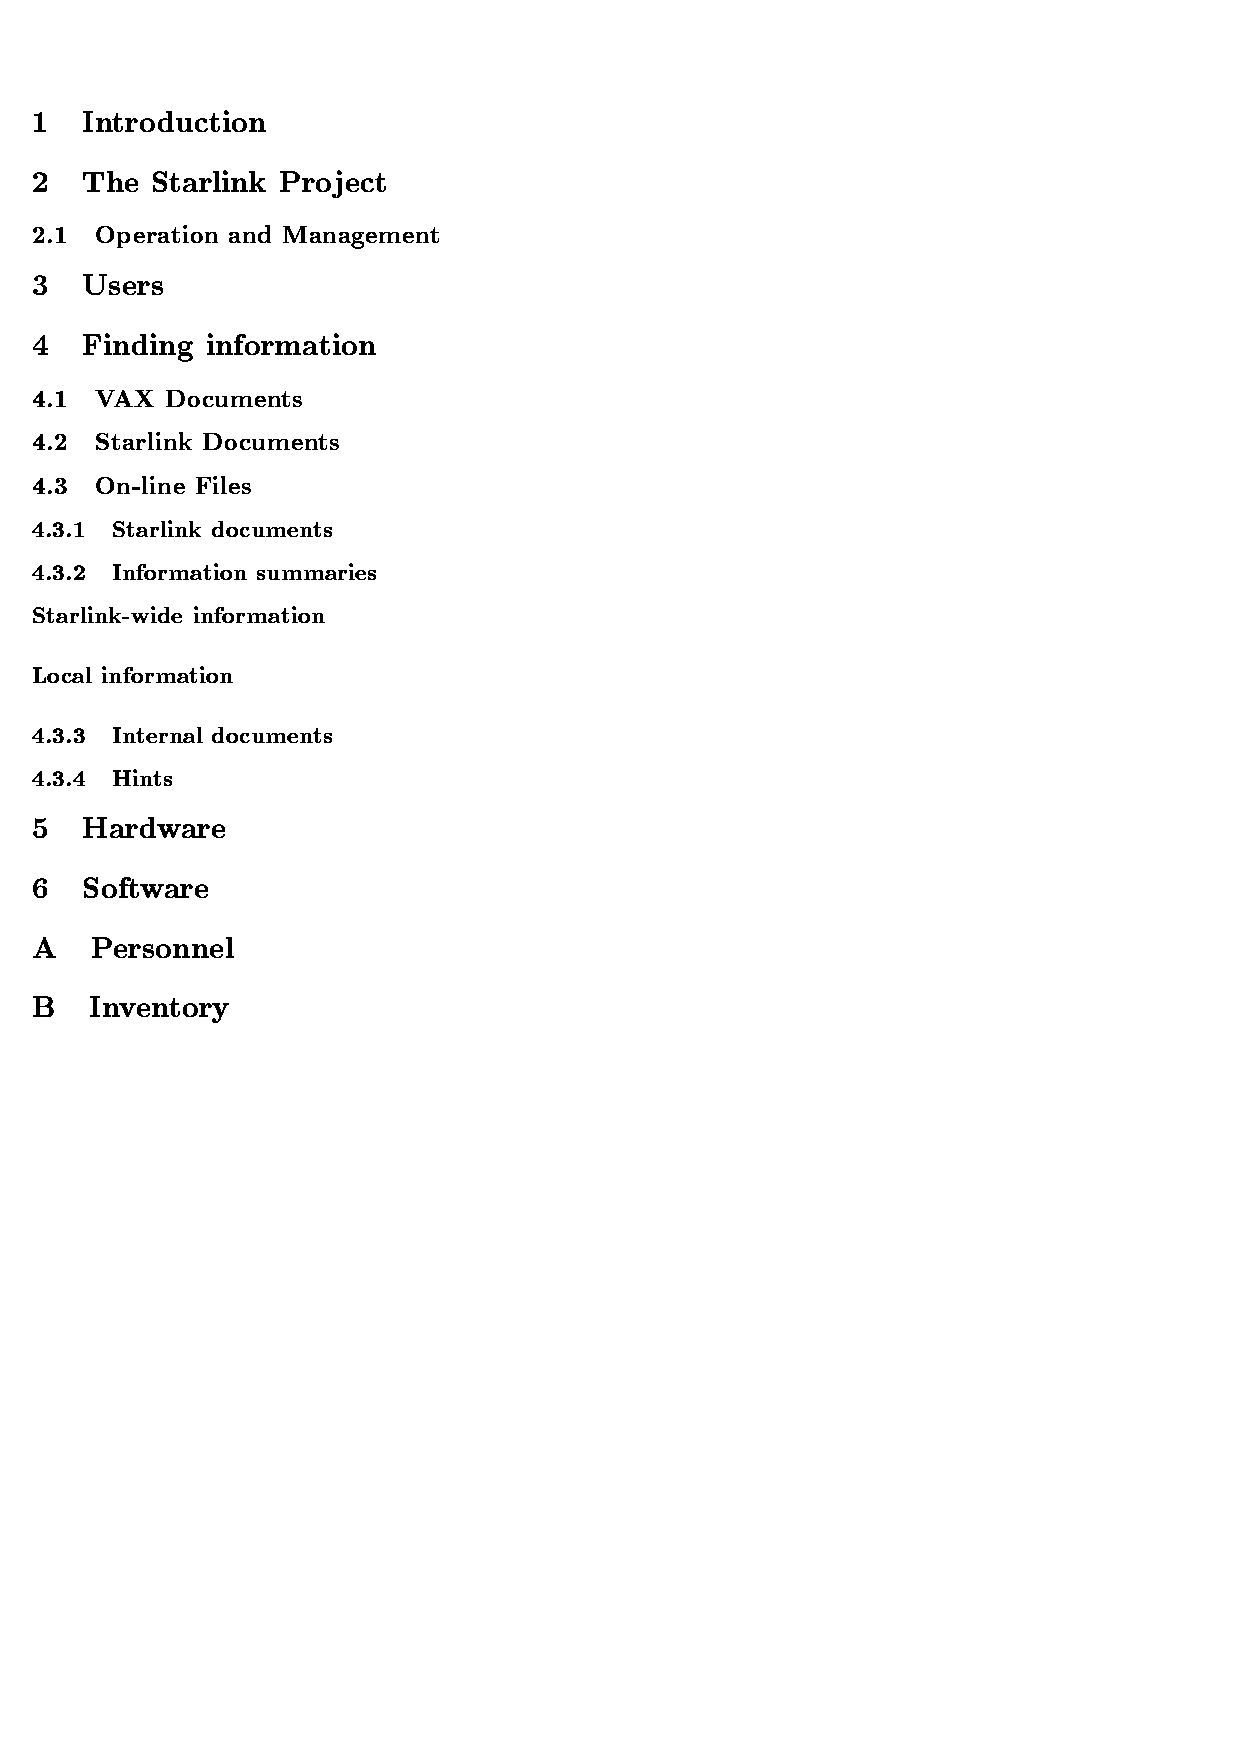
\includegraphics[viewport=0 350 215 842]{sc9a}
  \end{figure}
\end{center}

\newpage

\section{Font size and type\xlabel{font_size_and_type}}

\begin{small}
\begin{terminalv}
You can use a large number of different sizes and types of font.
This is the one you get by default.

\vspace{10mm}

\begin{quote}

\textrm{This is Rom style --- 1 2 3 4.}

\emph{This is Emph style --- 1 2 3 4.}

\textbf{This is Bold style --- 1 2 3 4.}

\textit{This is Ital style --- 1 2 3 4.}

\textsl{This is Slan style --- 1 2 3 4.}

\textsf{This is SSrf style --- 1 2 3 4.}

\textsc{This is caps style --- 1 2 3 4.}

\\texttt{This is Type style --- 1 2 3 4.}

{\tiny This is tiny size.}

{\scriptsize This is scriptsize.}

{\footnotesize This is footnotesize.}

{\small This is small size.}

{\normalsize This is normalsize.}

{\large This is large size.}

{\Large This is Large size.}

{\LARGE This is LARGE size.}

{\huge This is huge size.}

{\Huge This is Huge size.}

\end{quote}

\vspace{10mm}

The full selection of fonts available is illustrated in \xref{SUN/93}{sun93}{}.
\end{terminalv}
\end{small}

\newpage

\begin{center}
\textbf{\LaTeX\ OUTPUT}
\end{center}

You can use a large number of different sizes and types of font.
This is the one you get by default.

\vspace{10mm}

\begin{quote}

\textrm{This is Rom style --- 1 2 3 4.}

\emph{This is Emph style --- 1 2 3 4.}

\textbf{This is Bold style --- 1 2 3 4.}

\textit{This is Ital style --- 1 2 3 4.}

\textsl{This is Slan style --- 1 2 3 4.}

\textsf{This is SSrf style --- 1 2 3 4.}

\textsc{This is caps style --- 1 2 3 4.}

\texttt{This is Type style --- 1 2 3 4.}

{\tiny This is tiny size.}

{\scriptsize This is scriptsize.}

{\footnotesize This is footnotesize.}

{\small This is small size.}

{\normalsize This is normalsize.}

{\large This is large size.}

{\Large This is Large size.}

{\LARGE This is LARGE size.}

{\huge This is huge size.}

{\Huge This is Huge size.}

\end{quote}

\vspace{10mm}

The full selection of fonts available is illustrated in \xref{SUN/93}{sun93}{}.

\newpage

\section{Lists\xlabel{lists}}

\footnotesize
\begin{terminalv}
Starlink staff:
\begin{itemize}
  \item manage the project.
  \item support users and programmers.
  \begin{itemize}
    \item answer the phone.
    \item answer mail messages.
    \item soothe those having a nervous breakdown.
  \end{itemize}
  \item maintain contact with other astronomical groups.
\end{itemize}

******************************************************************************

FIELDNAMEs used in the CAR system are:
\begin{description}
  \item [TITLE] -
  This contains the name of the catalogue and is mandatory.
  FORMAT2 should be A.
  VALUE should be a mnemonic ($<$6 characters).
  COMMENT should be the ordinary title.
  \item [MEDIUM] -
  This is the storage medium of the data and is mandatory.
  FORMAT2 should be A.
  VALUE should be:
  \begin{description}
    \item [TAPE] -
    to select magnetic tape.
    \item [DISK] -
    to select disk.
  \end{description}
  \item [ACCESSMODE] -
  This is the mode of getting records from and putting them into the file.
  FORMAT2 should be A.
  VALUE should be SEQUENTIAL, DIRECT or KEYED; the latter is for access to
  Indexed Sequential Accessmode Files.
  ACCESSMODE is mandatory when MEDIUM is DISK.
\end{description}

******************************************************************************

This is an invitation to input one of the following:
\begin{enumerate}
  \item The name of an application program,
  \item The name of a ICL procedure,
  \begin{enumerate}
    \item Actual name
    \item Logical name
  \end{enumerate}
  \item A ICL command
\end{enumerate}
with an optional argument list.
In cases 1 and 2 a search is carried out for the executable image file or
procedure file.
\end{terminalv}
\normalsize

\newpage

\begin{center}
  \textbf{\LaTeX\ OUTPUT}
\end{center}

Starlink staff:
\begin{itemize}
  \item manage the project.
  \item support users and programmers.
  \begin{itemize}
    \item answer the phone.
    \item answer mail messages.
    \item soothe those having a nervous breakdown.
  \end{itemize}
  \item maintain contact with other astronomical groups.
\end{itemize}

******************************************************************************

FIELDNAMEs used in the CAR system are:
\begin{description}
  \item [TITLE] -
  This contains the name of the catalogue and is mandatory.
  FORMAT2 should be A.
  VALUE should be a mnemonic ($<$6 characters).
  COMMENT should be the ordinary title.
  \item [MEDIUM] -
  This is the storage medium of the data and is mandatory.
  FORMAT2 should be A.
  VALUE should be:
  \begin{description}
    \item [TAPE] -
    to select magnetic tape.
    \item [DISK] -
    to select disk.
  \end{description}
  \item [ACCESSMODE] -
  This is the mode of getting records from and putting them into the file.
  FORMAT2 should be A.
  VALUE should be SEQUENTIAL, DIRECT or KEYED; the latter is for access to
  Indexed Sequential Accessmode Files.
  ACCESSMODE is mandatory when MEDIUM is DISK.
\end{description}

******************************************************************************

This is an invitation to input one of the following:
\begin{enumerate}
  \item The name of an application program,
  \item The name of a DSCL procedure,
  \begin{enumerate}
    \item Actual name
    \item Logical name
  \end{enumerate}
  \item A DSCL or DCL command
\end{enumerate}
with an optional argument list.
In cases 1 and 2 a search is carried out for the executable image file or
procedure file.

\newpage

\section{Displays\xlabel{displays}}

\begin{small}
\begin{terminalv}
There are three main areas of help information: CAR\_HELP for information
about the CAR routines; CAT\_HELP for information about the catalogues and
SCAR\_HELP for general information.
\end{terminalv}
\verb+\begin{terminalv}+
\begin{terminalv}
ICL> CAR_HELP
SCAR COMMANDS Subtopic? CAR_SEARCH
\end{terminalv}
\verb+\end{terminalv}+
\begin{terminalv}
You would find information about the CAR\_SEARCH procedure.
\end{terminalv}
\verb+\begin{terminalv}+
\begin{terminalv}
ICL> CAT_HELP
Topic? $Summary
\end{terminalv}
\verb+\end{terminalv}+
\begin{terminalv}
The catalogues are summarised in this help library.
The acronym for the IRAS point source catalogue is IRPS.

******************************************************************************

The parameters\footnote{By the way, this is how to insert a footnote} before
the `;' are input parameters; those after are output parameters.
Routines belonging to the HDS kernel are identified by the symbol `[K]'.

\noindent
\textbf{CMP\_GET0x}\emph{(loc,name;value,status)} --- Read scalar component\\
\textbf{CMP\_GET1x}\emph{(loc,name,elx;value,el,status)} --- Read vector component\\
\textbf{CMP\_GETNx}\emph{(loc,name,ndim,dimx;value,dim,status)} --- Read array
component\\
\textbf{CMP\_GETVx}\emph{(loc,name,elx;value,el,status)} --- Read vectorised
component\\
\textbf{CMP\_LEN}\emph{(loc,name;len,status)} --- Enquire component precision\\

******************************************************************************

These are the catalogues online at RAL, (R = Access restricted):
\begin{quote}
  \begin{description}
    \item [AIPS] -- Associations of IRAS point sources.
    \item [AS85] -- CHART Astrometry catalogue.
    \item [ASIR] -- Global Index for AIPS and IRPS.
    \item [ASSC] -- Associations of IRAS Small Scale Structure Catalogue.
    \item [CATX] -- Catalogue X: Merger of UGC, ESOB, CGCG.
    \item [CSIS] -- CHART CSI 1979 Version.
  \end{description}
\end{quote}
\end{terminalv}
\end{small}

\newpage

\begin{center}
  \textbf{\LaTeX\ OUTPUT}
\end{center}

There are three main areas of help information: CAR\_HELP for information
about the CAR routines; CAT\_HELP for information about the catalogues and
SCAR\_HELP for general information.
\begin{terminalv}
ICL> CAR_HELP
SCAR COMMANDS Subtopic? CAR_SEARCH
\end{terminalv}
You would find information about the CAR\_SEARCH procedure.
\begin{terminalv}
ICL> CAT_HELP
Topic? $Summary
\end{terminalv}
The catalogues are summarised in this help library.
The acronym for the IRAS point source catalogue is IRPS.


******************************************************************************

The parameters\footnote{By the way, this is how to insert a footnote} before
the `;' are input parameters; those after are output parameters.
Routines belonging to the HDS kernel are identified by the symbol `[K]'.

\noindent
\textbf{CMP\_GET0x}\emph{(loc,name;value,status)} --- Read scalar component\\
\textbf{CMP\_GET1x}\emph{(loc,name,elx;value,el,status)} --- Read vector component\\
\textbf{CMP\_GETNx}\emph{(loc,name,ndim,dimx;value,dim,status)} --- Read array
component\\
\textbf{CMP\_GETVx}\emph{(loc,name,elx;value,el,status)} --- Read vectorised
component\\
\textbf{CMP\_LEN}\emph{(loc,name;len,status)} --- Enquire component precision\\

******************************************************************************

These are the catalogues online at RAL, (R = Access restricted):
\begin{quote}
  \begin{description}
    \item [AIPS] -- Associations of IRAS point sources.
    \item [AS85] -- CHART Astrometry catalogue.
    \item [ASIR] -- Global Index for AIPS and IRPS.
    \item [ASSC] -- Associations of IRAS Small Scale Structure Catalogue.
    \item [CATX] -- Catalogue X: Merger of UGC, ESOB, CGCG.
    \item [CSIS] -- CHART CSI 1979 Version.
  \end{description}
\end{quote}

\newpage

\begin{footnotesize}
\begin{terminalv}
The error status code symbol is constructed by concatenating the string
`ERR\_' with an error code.
The error codes and their meanings are listed below:
\begin{description}
  \item [DIMINV]:
  \emph{Dimensions invalid (out-of-range)}.
  It is likely that certain groups of users will be restricted in the size of the
  frames they can access.
  RDIMAG and WRIMAG return this status if the user has insufficient quota to map
  the frame.
  This status will also be set when attempting to create an output frame of a
  negative or zero size.
  \item [DSCNPR]:
  \emph{Descriptor item not present}.
  For DLDSCR and RDDSCR, the specified descriptor item name cannot be found within
  the frame's descriptor.
  For RDDSCN, no item can be found with the specified name as the end of the
  descriptor list was encountered.
\end{description}

******************************************************************************

This program allows you to specify fields within any catalogue and then perform
statistical analysis on the selected fields(s).
\begin{description}
  \item [ANALYSE/HISTOGRAM] --
  This is option 1 on the first menu.
  You will be prompted for the name of the input catalogue and the name of the
  field to be analysed.
  The field values are read in from the catalogue and the mean, mode standard
  deviation, maximum and minimum values are presented to you.
  You can identify any statistic by looking up HIST in the help libraries.
  You should note X\_MAX, X\_MIN and MODE\_SZ for designing the axis scales of
  your plot.
  \begin{description}
    \item [Prompts] --
    \begin{description}
      \item [STYLE] -- The user selection from a menu.
      The expected input is an integer and ranges from the values shown on the menu.
      \item [INPUT] -- The name of the catalogue from which the field is to be taken.
      \item [PTYPE] - The type of plot you want; this is either a connected point graph or
      a standard histogram.
    \end{description}
  \end{description}
  \item [ANALYSE/SCATTERPLOT] --
  This is option 2 on the first menu.
  Linear regression is performed on the two specified fields and then a scatter
  diagram with the line of best fit is plotted.
  \begin{description}
    \item [Prompts] --
    \begin{description}
      \item [STYLE]-- Select from a menu; the expected input is an integer
      and ranges from the values shown on the menu.
      \item [INPUT] -- The name of the catalogue from which the field is to be taken.
    \end{description}
  \end{description}
\end{description}
\end{terminalv}
\end{footnotesize}

\newpage

\begin{center}
  \textbf{\LaTeX\ OUTPUT}
\end{center}

The error status code symbol is constructed by concatenating the string
`ERR\_' with an error code.
The error codes and their meanings are listed below:
\begin{description}
  \item [DIMINV]:
  \emph{Dimensions invalid (out-of-range)}.
  It is likely that certain groups of users will be restricted in the size of the
  frames they can access.
  RDIMAG and WRIMAG return this status if the user has insufficient quota to map
  the frame.
  This status will also be set when attempting to create an output frame of a
  negative or zero size.
  \item [DSCNPR]:
  \emph{Descriptor item not present}.
  For DLDSCR and RDDSCR, the specified descriptor item name cannot be found within
  the frame's descriptor.
  For RDDSCN, no item can be found with the specified name as the end of the
  descriptor list was encountered.
\end{description}

******************************************************************************

This program allows you to specify fields within any catalogue and then perform
statistical analysis on the seclected fields(s).
\begin{description}
  \item [ANALYSE/HISTOGRAM] --
  This is option 1 on the first menu.
  You will be prompted for the name of the input catalogue and the name of the
  field to be analysed.
  The field values are read in from the catalogue and the mean, mode standard
  deviation, maximum and minimum values are presented to you.
  You can identify any statistic by looking up HIST in the help libraries.
  You should note X\_MAX, X\_MIN and MODE\_SZ for designing the axis scales of
  your plot.
  \begin{description}
    \item [Prompts] --
    \begin{description}
      \item [STYLE] -- The user selection from a menu.
      The expected input is an integer and ranges from the values shown on the menu.
      \item [INPUT] -- The name of the catalogue from which the field is to be taken.
      \item [PTYPE] - The type of plot you want; this is either a connected point graph or
      a standard histogram.
    \end{description}
  \end{description}
  \item [ANALYSE/SCATTERPLOT] --
  This is option 2 on the first menu.
  Linear regression is performed on the two specified fields and then a scatter
  diagram with the line of best fit is plotted.
  \begin{description}
    \item [Prompts] --
    \begin{description}
      \item [STYLE]-- Select from a menu; the expected input is an integer
      and ranges from the values shown on the menu.
      \item [INPUT] -- The name of the catalogue from which the field is to be taken.
    \end{description}
  \end{description}
\end{description}
\newpage

\section{Routine specifications\xlabel{routine_specifications}}

\small
\begin{terminalv}
This appendix documents the INTERIM routines in alphabetical order.\\
\rule{\textwidth}{0.3mm}
{\Large \textbf{ADDSCR} \hfill Add Descriptor Item \hfill \textbf{ADDSCR}}
\begin{description}
  \item [FUNCTION]:
  Writes a new item in a frame descriptor.
  In general, the item value is a vector of elements.
  If  an item with the same name already exists in the descriptor, the supplied
  elements are appended to the existing ones.
  \item [CALL]:
  \begin{quote}
    \texttt{ CALL ADDSCR(name,descr,value,nels,status)}
  \end{quote}
  \item [INPUT ARGUMENTS]:
  \begin{tabbing}
    descrxxx\=CHARACTERx\=expressionxxx\=\kill
    \emph{name}\>CHARACTER\>expression\>Parameter name (FRAME class).\\
    \emph{descr}\>CHARACTER\>expression\>Descriptor item name.\\
    \emph{value}\>CHARACTER\>array\>Element values.\\
    \emph{nels}\>INTEGER\>expression\>Number of elements in \emph{value}.
  \end{tabbing}
  \item [OUTPUT ARGUMENT]:
  \begin{tabbing}
    descrxxx\=CHARACTERx\=expressionxxx\=\kill
    \emph{status}\>INTEGER\>variable\>Status return.
  \end{tabbing}
\end{description}
\goodbreak
\rule{\textwidth}{0.3mm}
{\Large \textbf{DLDSCR} \hfill Delete Descriptor Item \hfill \textbf{DLDSCR}}
\begin{description}
  \item [FUNCTION]:
  Deletes an existing descriptor item from a frame.
  \item [CALL]:
  \begin{quote}
    \texttt{ CALL DLDSCR(name,descr,status)}
  \end{quote}
  \item [INPUT ARGUMENTS]:
  \begin{tabbing}
    descrxxx\=CHARACTERx\=expressionxxx\=\kill
    \emph{name}\>CHARACTER\>expression\>Parameter name (FRAME class).\\
    \emph{descr}\>CHARACTER\>expression\>Descriptor item name.
  \end{tabbing}
  \item [OUTPUT ARGUMENT]:
  \begin{tabbing}
    descrxxx\=CHARACTERx\=expressionxxx\=\kill
    \emph{status}\>INTEGER\>variable\>Status return.
  \end{tabbing}
\end{description}
\goodbreak
\end{terminalv}
\normalsize

\newpage

\begin{center}
  \textbf{\LaTeX\ OUTPUT}
\end{center}

This appendix documents the INTERIM routines in alphabetical order.\\
\rule{\textwidth}{0.3mm}
{\Large \textbf{ADDSCR} \hfill Add Descriptor Item \hfill \textbf{ADDSCR}}
\begin{description}
  \item [FUNCTION]:
  Writes a new item in a frame descriptor.
  In general, the item value is a vector of elements.
  If  an item with the same name already exists in the descriptor, the supplied
  elements are appended to the existing ones.
  \item [CALL]:
  \begin{quote}
    \texttt{ CALL ADDSCR(name,descr,value,nels,status)}
  \end{quote}
  \item [INPUT ARGUMENTS]:
  \begin{tabbing}
    descrxxx\=CHARACTERx\=expressionxxx\=\kill
    \emph{name}\>CHARACTER\>expression\>Parameter name (FRAME class).\\
    \emph{descr}\>CHARACTER\>expression\>Descriptor item name.\\
    \emph{value}\>CHARACTER\>array\>Element values.\\
    \emph{nels}\>INTEGER\>expression\>Number of elements in \emph{value}.
  \end{tabbing}
  \item [OUTPUT ARGUMENT]:
  \begin{tabbing}
    descrxxx\=CHARACTERx\=expressionxxx\=\kill
    \emph{status}\>INTEGER\>variable\>Status return.
  \end{tabbing}
\end{description}
\goodbreak
\rule{\textwidth}{0.3mm}
{\Large \textbf{DLDSCR} \hfill Delete Descriptor Item \hfill \textbf{DLDSCR}}
\begin{description}
  \item [FUNCTION]:
  Deletes an existing descriptor item from a frame.
  \item [CALL]:
  \begin{quote}
    \texttt{ CALL DLDSCR(name,descr,status)}
  \end{quote}
  \item [INPUT ARGUMENTS]:
  \begin{tabbing}
    descrxxx\=CHARACTERx\=expressionxxx\=\kill
    \emph{name}\>CHARACTER\>expression\>Parameter name (FRAME class).\\
    \emph{descr}\>CHARACTER\>expression\>Descriptor item name.
  \end{tabbing}
  \item [OUTPUT ARGUMENT]:
  \begin{tabbing}
    descrxxx\=CHARACTERx\=expressionxxx\=\kill
    \emph{status}\>INTEGER\>variable\>Status return.
  \end{tabbing}
\end{description}
\goodbreak

\newpage

\section{Mathematics\xlabel{mathematics}}

\begin{terminalv}
The optional globular cluster is generated using a King (1962)
star density law
\begin{equation}
  D(r)=k((1+(r/r_{c})^{2})^{-1/2}-(1+(r_{t}/r_{c})^{2})^{-1/2})^{2}
\end{equation}
where $D(r)$ is the star surface density a projected distance $r$ from the
centre of the cluster.
$k$, $r_{c}$ and $r_{t}$ are constants, $k$ being a scale factor and $r_{c}$
and $r_{t}$ the core and tidal radii respectively.

Moffat's formula gives the intensity I(r) at a radial distance r from the
centre of the star image as
\begin{equation}
  I(r)=I_{0}/(1+(\frac{r}{R})^{2})^{\beta}
\end{equation}
where $I_{0}$, R and $\beta$ are all constants.
The total luminosity, Lt, of such a profile is
\begin{equation}
  Lt=\frac{\pi R^{2}I_{0}}{\beta -1}
\end{equation}
so
\begin{equation}
  I(r)=\frac{Lt(\beta -1)}{\pi^{2}R^{2}}/(1+(\frac{r}{R})^{2})^{\beta}
\end{equation}

If the intensity threshold beyond which the profile is truncated is $I_{th}$,
then the corresponding radius $r_{th}$ is
\begin{equation}
  r_{th}=((\frac{Lt(\beta -1)}{I_{th}\pi R^{2}})^{1/\beta}-1)^{1/2}R
\end{equation}
from this, the fraction of the total light emitted beyond this boundary, f, may
be calculated
\begin{equation}
  f=(1+(\frac{r_{th}}{R})^{2})^{1-\beta}
\end{equation}
\begin{displaymath}
  B=\frac {\pi( (X-(\frac{IXEXT}{2}-1))^{2} +
  (Y-\frac{IYEXT}{2})^{2} )^{\frac{1}{2}}} {A}
\end{displaymath}
\end{terminalv}

\newpage

\begin{center}
  \textbf{\LaTeX\ OUTPUT}
\end{center}

The optional globular cluster is generated using a King (1962)
star density law
\begin{equation}
  D(r)=k((1+(r/r_{c})^{2})^{-1/2}-(1+(r_{t}/r_{c})^{2})^{-1/2})^{2}
\end{equation}
where $D(r)$ is the star surface density a projected distance $r$ from the
centre of the cluster.
$k$, $r_{c}$ and $r_{t}$ are constants, $k$ being a scale factor and $r_{c}$
and $r_{t}$ the core and tidal radii respectively.

Moffat's formula gives the intensity I(r) at a radial distance r from the
centre of the star image as
\begin{equation}
  I(r)=I_{0}/(1+(\frac{r}{R})^{2})^{\beta}
\end{equation}
where $I_{0}$, R and $\beta$ are all constants.
The total luminosity, Lt, of such a profile is
\begin{equation}
  Lt=\frac{\pi R^{2}I_{0}}{\beta -1}
\end{equation}
so
\begin{equation}
  I(r)=\frac{Lt(\beta -1)}{\pi^{2}R^{2}}/(1+(\frac{r}{R})^{2})^{\beta}
\end{equation}

If the intensity threshold beyond which the profile is truncated is $I_{th}$,
then the corresponding radius $r_{th}$ is
\begin{equation}
  r_{th}=((\frac{Lt(\beta -1)}{I_{th}\pi R^{2}})^{1/\beta}-1)^{1/2}R
\end{equation}
from this, the fraction of the total light emitted beyond this boundary, f, may
be calculated
\begin{equation}
  f=(1+(\frac{r_{th}}{R})^{2})^{1-\beta}
\end{equation}
\begin{displaymath}
  B=\frac {\pi( (X-(\frac{IXEXT}{2}-1))^{2} +
  (Y-\frac{IYEXT}{2})^{2} )^{\frac{1}{2}}} {A}
\end{displaymath}

\newpage

\begin{terminalv}
An AR model is of the form
\begin{equation}
  X_{i}=\sum_{j=1}^{M} A_{j}X_{i-j}+E_{i}
\end{equation}
for equally spaced observations $X_{i}$ and for a set of constants $A_{j}$.
$E_{i}$ is the error in using this model.
The method involves choosing the $A_{j}$ to minimize the $E_{i}$.

The Q, U and E frames can now be calculated as follows:
\[Q_{ij}=\frac{A_{ij}-B_{ij}}{A_{ij}+B_{ij}}\]
\[U_{ij}=\frac{C_{ij}-D_{ij}}{C_{ij}+D_{ij}}\]
\[E_{ij}=\frac{2}{A_{ij}+B_{ij}+C_{ij}+D_{ij}}\]
The total polarization frame, P, and polarization angle frame, T, are generated
from Q, U and (if required) E as follows:
\[P_{ij}=\sqrt{{Q_{ij}}^{2}+{U_{ij}}^{2}}-E_{ij}\]
\[T_{ij}=0.5\arctan \frac{U_{ij}}{Q_{ij}}\]
The values of Tij are restricted to the range 0 to +$\pi$ radians.

Every pixel (X,Y) in the image frame is multiplied by SIN(B)/B where
\begin{displaymath}
  B=\frac {\pi( (X-(\frac{IXEXT}{2}-1))^{2} +
  (Y-\frac{IYEXT}{2})^{2} )^{\frac{1}{2}}} {A}
\end{displaymath}
\end{terminalv}

\newpage

\begin{center}
  \textbf{\LaTeX\ OUTPUT}
\end{center}

An AR model is of the form
\begin{equation}
  X_{i}=\sum_{j=1}^{M} A_{j}X_{i-j}+E_{i}
\end{equation}
for equally spaced observations $X_{i}$ and for a set of constants $A_{j}$.
$E_{i}$ is the error in using this model.
The method involves choosing the $A_{j}$ to minimize the $E_{i}$.

The Q, U and E frames can now be calculated as follows:
\[Q_{ij}=\frac{A_{ij}-B_{ij}}{A_{ij}+B_{ij}}\]
\[U_{ij}=\frac{C_{ij}-D_{ij}}{C_{ij}+D_{ij}}\]
\[E_{ij}=\frac{2}{A_{ij}+B_{ij}+C_{ij}+D_{ij}}\]
The total polarization frame, P, and polarization angle frame, T, are generated
from Q, U and (if required) E as follows:
\[P_{ij}=\sqrt{{Q_{ij}}^{2}+{U_{ij}}^{2}}-E_{ij}\]
\[T_{ij}=0.5\arctan \frac{U_{ij}}{Q_{ij}}\]
The values of Tij are restricted to the range 0 to +$\pi$ radians.

Every pixel (X,Y) in the image frame is multiplied by SIN(B)/B where
\begin{displaymath}
  B=\frac {\pi( (X-(\frac{IXEXT}{2}-1))^{2} +
  (Y-\frac{IYEXT}{2})^{2} )^{\frac{1}{2}}} {A}
\end{displaymath}
\newpage

\section{Tabbing\xlabel{tabbing}}

\begin{terminalv}
\begin{quote}
  \begin{tabbing}
    ROUTINExxx\=ERRxFMTBADxx\==x8xxxx\=\kill
    \textbf{ROUTINE}\>\textbf{SYMBOL}\>\>\textbf{MEANING}\\
    \\
    ADDSCR:\>ERR\_FRMNUL\>= 1\>Frame null.\\
    \>ERR\_FRMNAC\>= 3\>Frame could not be accessed.\\
    \>ERR\_PARINV\>= 4\>Parameter name invalid.\\
    \\
    CNPAR:\>ERR\_PARANC\>= 2\>Parameter association not cancelled.\\
    \>ERR\_PARINV\>= 4\>Parameter name invalid.\\
    \\
    CTOI:\>ERR\_INPINV\>= 5\>Input invalid.\\
    \\
    CTOR:\>ERR\_INPINV\>= 5\>Input invalid.\\
  \end{tabbing}
\end{quote}

******************************************************************************

\begin{tabbing}
  namexx\=positionxx\=maxdimsxx\=dimensxx\=pointerxx\=pointerxxx\=\kill
  \emph{name}\>\emph{default}\>\emph{maxels}\>\emph{value}\>\emph{actels}
    \>\>\textbf{RDKEYx}\\
  \emph{name}\>\>\>\emph{value}\>\emph{nels}\>\>\textbf{WRKEYx}\\
  \\
  \emph{name}\>\emph{dtype}\>\emph{ftype}\>\emph{size}\>\emph{pointer}
    \>\>\textbf{RDDATA, WRDATA}\\
  \emph{name}\>\emph{dtype}\>\>\emph{size}\>\emph{pointer}\>\>\textbf{GETDYN}\\
  \\
  \emph{name}\>\emph{dtype}\>\emph{maxdims}\>\emph{dimens}\>\emph{actdims}
    \>\emph{pointer}\>\textbf{RDIMAG}\\
  \emph{name}\>\emph{dtype}\>\>\emph{dimens}\>\emph{ndims}\>\emph{pointer}
    \>\textbf{WRIMAG}\\
\end{tabbing}
\end{terminalv}

\newpage

\begin{center}
  \textbf{\LaTeX\ OUTPUT}
\end{center}

\begin{quote}
  \begin{tabbing}
    ROUTINExxx\=ERRxFMTBADxx\==x8xxxx\=\kill
    \textbf{ROUTINE}\>\textbf{SYMBOL}\>\>\textbf{MEANING}\\
    \\
    ADDSCR:\>ERR\_FRMNUL\>= 1\>Frame null.\\
    \>ERR\_FRMNAC\>= 3\>Frame could not be accessed.\\
    \>ERR\_PARINV\>= 4\>Parameter name invalid.\\
    \\
    CNPAR:\>ERR\_PARANC\>= 2\>Parameter association not cancelled.\\
    \>ERR\_PARINV\>= 4\>Parameter name invalid.\\
    \\
    CTOI:\>ERR\_INPINV\>= 5\>Input invalid.\\
    \\
    CTOR:\>ERR\_INPINV\>= 5\>Input invalid.\\
  \end{tabbing}
\end{quote}

******************************************************************************

\begin{tabbing}
  namexx\=positionxx\=maxdimsxx\=dimensxx\=pointerxx\=pointerxxx\=\kill
  \emph{name}\>\emph{default}\>\emph{maxels}\>\emph{value}\>\emph{actels}
    \>\>\textbf{RDKEYx}\\
  \emph{name}\>\>\>\emph{value}\>\emph{nels}\>\>\textbf{WRKEYx}\\
  \\
  \emph{name}\>\emph{dtype}\>\emph{ftype}\>\emph{size}\>\emph{pointer}
    \>\>\textbf{RDDATA, WRDATA}\\
  \emph{name}\>\emph{dtype}\>\>\emph{size}\>\emph{pointer}\>\>\textbf{GETDYN}\\
  \\
  \emph{name}\>\emph{dtype}\>\emph{maxdims}\>\emph{dimens}\>\emph{actdims}
    \>\emph{pointer}\>\textbf{RDIMAG}\\
  \emph{name}\>\emph{dtype}\>\>\emph{dimens}\>\emph{ndims}\>\emph{pointer}
    \>\textbf{WRIMAG}\\
\end{tabbing}

\newpage

\small
\begin{terminalv}
The following qualifiers are recognized:

\begin{list}{}{\settowidth{\labelwidth}{\texttt{-f}\emph{filename}}
  \setlength{\leftmargin}{\labelwidth}
  \addtolength{\labelwidth}{\labelsep}}
  \item[\texttt{-b}] Process pages in reverse order; this can be useful on the
  A2 model printers which stack their pages face up and therefore in the
  reverse of the order in which they were printed.
  \item[\texttt{-c\#}]  Print \texttt{\#} copies of each page; a photocopier is
  cheaper so this qualifier shouldn't really be needed.
  \item[\texttt{-x\#}\textit{unit}] Set the left margin to \texttt{\#} (which
  can be both a real number and negative); \textit{unit} is one of:

  \begin{tabular}{ll}
    bp &big point (1in = 72bp)\\
    cc &cicero (1cc = 12dd)\\
    cm &centimetre (1in = 2.54cm)\\
    dd &didot point (1157dd = 1238pt)\\
    in &inch\\
    mm &millimetre\\
    pc &pica (1pc = 12pt)\\
    pt &point (72.27pt = 1in)\\
    sp &scaled point (65536sp = 1pt)
  \end{tabular}

  The default margin is 1in.
  \item[\texttt{-y\#}\textit{unit}] Set top margin. The default is 1in.
\end{list}

******************************************************************************

\newlength{\numlen}
\settowidth{\numlen}{xxxx000--000--0000}
\settowidth{\labelsep}{000}

\begin{list}{}{\setlength{\labelwidth}{\numlen}\setlength{\leftmargin}{\numlen}
  \addtolength{\leftmargin}{\labelsep}}
  \item[0385--41191] (RDC) V21, (use 8-bit no-parity), connected to
  Departmental Gandalf PACX.
  PACX service is \texttt{STARN}.
  More details if you specify \texttt{HELP} instead of \texttt{STARN} after
  the Gandalf prompt.
  \item[061--273--5730] (RDC) V21/V23 (autobaud), seven bits, even parity,
  connected to VAX--11/750.
  \item[0477--71324] (RDC) V21/V23/V22/V22bis (autobaud), connected to a DECserver
  200.
  \item[0235--831--593] (RDC) VAX 11/780, V22.
  \item[0235--44--6951] PAD line V21/V23.
  \item[0235--44--6952] PAD line V22/V22bis.
\end{list}
\end{terminalv}
\normalsize

\newpage

\begin{center}
  \textbf{\LaTeX\ OUTPUT}
\end{center}

The following qualifiers are recognized:

\begin{list}{}{\settowidth{\labelwidth}{\texttt{-f}\emph{filename}}
  \setlength{\leftmargin}{\labelwidth}
  \addtolength{\labelwidth}{\labelsep}}
  \item[\texttt{-b}] Process pages in reverse order; this can be useful on the
  A2 model printers which stack their pages face up and therefore in the
  reverse of the order in which they were printed.
  \item[\texttt{-c\#}]  Print \texttt{\#} copies of each page; a photocopier is
  cheaper so this qualifier shouldn't really be needed.
  \item[\texttt{-x\#}\textit{unit}] Set the left margin to \texttt{\#} (which
  can be both a real number and negative); \textit{unit} is one of:

  \begin{tabular}{ll}
    bp &big point (1in = 72bp)\\
    cc &cicero (1cc = 12dd)\\
    cm &centimetre (1in = 2.54cm)\\
    dd &didot point (1157dd = 1238pt)\\
    in &inch\\
    mm &millimetre\\
    pc &pica (1pc = 12pt)\\
    pt &point (72.27pt = 1in)\\
    sp &scaled point (65536sp = 1pt)
  \end{tabular}

  The default margin is 1in.
  \item[\texttt{-y\#}\textit{unit}] Set top margin. The default is 1in.
\end{list}

******************************************************************************

\newlength{\numlen}
\settowidth{\numlen}{xxxx000--000--0000}
\settowidth{\labelsep}{000}

\begin{list}{}{\setlength{\labelwidth}{\numlen}\setlength{\leftmargin}{\numlen}
  \addtolength{\leftmargin}{\labelsep}}
  \item[0385--41191] (RDC) V21, (use 8-bit no-parity), connected to
  Departmental Gandalf PACX.
  PACX service is \texttt{STARN}.
  More details if you specify \texttt{HELP} instead of \texttt{STARN} after
  the Gandalf prompt.
  \item[061--273--5730] (RDC) V21/V23 (autobaud), seven bits, even parity,
  connected to VAX--11/750.
  \item[0477--71324] (RDC) V21/V23/V22/V22bis (autobaud), connected to a DECserver
  200.
  \item[0235--831--593] (RDC) VAX 11/780, V22.
  \item[0235--44--6951] PAD line V21/V23.
  \item[0235--44--6952] PAD line V22/V22bis.
\end{list}

\newpage

\section{Tables\xlabel{tables}}

\begin{footnotesize}
\begin{terminalv}
\begin{table}
  \begin{center}
    \begin{tabular}{||c|c|c||} \hline
      \emph{ACCESS MODE} & \multicolumn{2}{c||}{\emph{MEDIUM}} \\ \cline{2-3}
      & \emph{Disk} & \emph{Tape} \\ \hline
      \emph{Sequential} & -- & BLOCKSIZE \\
      & & FILENUMBER \\ \hline
      \emph{Direct} & NRECORDS & -- \\
      & KEYFIELD & \\ \hline
    \end{tabular}
    \caption{Parameters required for access mode and medium}
  \end{center}
\end{table}

******************************************************************************

\begin{table}
  \begin{center}
    \begin{tabular}{||l|l|l||}
      \hline
      Primitive data type& VAX FORTRAN type	& HDS type \\
      \hline
      Integer			& \texttt{ INTEGER}	& \texttt{ `\_INTEGER'} \\
      Single floating point	& \texttt{ REAL}	& \texttt{ `\_REAL'} \\
      Double floating point& \texttt{ DOUBLE PRECISION} & \texttt{ `\_DOUBLE'} \\
      Logical	& \texttt{ LOGICAL}		& \texttt{ `\_LOGICAL'} \\
      Character	& \texttt{ CHARACTER[*n]}	& \texttt{ `\_CHAR[*n]'} \\
      \hline
    \end{tabular}
    \caption{Standard Primitive Data Types}
  \end{center}
\end{table}
\end{terminalv}
\end{footnotesize}

\newpage

\begin{center}
  \textbf{\LaTeX\ OUTPUT}
\end{center}

\begin{table}[h]
  \begin{center}
    \begin{tabular}{||c|c|c||} \hline
      \emph{ACCESS MODE} & \multicolumn{2}{c||}{\emph{MEDIUM}} \\ \cline{2-3}
& \emph{Disk} & \emph{Tape} \\ \hline
      \emph{Sequential} & -- & BLOCKSIZE \\
& & FILENUMBER \\ \hline
      \emph{Direct} & NRECORDS & -- \\
& KEYFIELD & \\ \hline
    \end{tabular}
    \caption{Parameters required for access mode and medium}
  \end{center}
\end{table}

******************************************************************************

\begin{table}[h]
  \begin{center}
    \begin{tabular}{||l|l|l||}
      \hline
      Primitive data type	& VAX FORTRAN type		& HDS type \\
      \hline
      Integer			& \texttt{ INTEGER}			& \texttt{ `\_INTEGER'} \\
      Single floating point	& \texttt{ REAL}			& \texttt{ `\_REAL'} \\
      Double floating point	& \texttt{ DOUBLE PRECISION}	& \texttt{ `\_DOUBLE'} \\
      Logical			& \texttt{ LOGICAL}			& \texttt{ `\_LOGICAL'} \\
      Character		& \texttt{ CHARACTER[*n]}		& \texttt{ `\_CHAR[*n]'} \\
      \hline
    \end{tabular}
    \caption{Standard Primitive Data Types}
  \end{center}
\end{table}

\newpage

\begin{footnotesize}
\begin{terminalv}
\begin{table}
  \begin{center}
    \begin{tabular}{|ll|ll|} \hline
      \multicolumn{2}{|c|}{\textbf{R.A.}}&\multicolumn{2}{c|}{\textbf{DEC.}} \\
      Accuracy used &Window size&Accuracy used &Window size\\ \hline
      Hours only&$\pm$30 mins&Degrees Only&$\pm$4 Degs\\
      Hours \& minutes&$\pm$10 mins&Degrees \& minutes &$\pm$25 mins\\
      Hours, mins \& secs&$\pm$30 Secs&Degrees, mins \& secs&$\pm$1 min\\ \hline
    \end{tabular}
  \end{center}
\end{table}

******************************************************************************

\begin{center}
  \begin{tabular}{c|p{33em}}
    \textbf{$<$fac$>$} & \textbf{Facility provides\ldots } \\
    \hline
    \\
    VAL & Arithmetic, mathematical functions and type conversion on single
    (scalar) \emph{values}.
    Handling of numerical errors and \emph{bad value} propagation are
    incorporated.\\
    \\
    VEC & Arithmetic, mathematical functions and type conversion on \emph{vectorised arrays},
          allowing more efficient processing of large numbers of
    data.
    Handling of numerical errors and \emph{bad value} propagation are
    incorporated.\\
    \\
  \end{tabular}
\end{center}
\end{terminalv}
\end{footnotesize}

\newpage

\begin{center}
  \textbf{\LaTeX\ OUTPUT}
\end{center}

\begin{table}[h]
  \begin{center}
    \begin{tabular}{|ll|ll|} \hline
      \multicolumn{2}{|c|}{\textbf{R.A.}}&\multicolumn{2}{c|}{\textbf{DEC.}} \\
      Accuracy used &Window size&Accuracy used &Window size\\ \hline
      Hours only&$\pm$30 mins&Degrees Only&$\pm$4 Degs\\
      Hours \& minutes&$\pm$10 mins&Degrees \& minutes &$\pm$25 mins\\
      Hours, mins \& secs&$\pm$30 Secs&Degrees, mins \& secs&$\pm$1 min\\ \hline
    \end{tabular}
  \end{center}
\end{table}

******************************************************************************

\begin{center}
  \begin{tabular}{c|p{33em}}
    \textbf{$<$fac$>$} & \textbf{Facility provides\ldots } \\
    \hline
    \\
    VAL & Arithmetic, mathematical functions and type conversion on single
    (scalar) \emph{values}.
    Handling of numerical errors and \emph{bad value} propagation are
    incorporated.\\
    \\
    VEC & Arithmetic, mathematical functions and type conversion on \emph{vectorised arrays}, allowing more efficient processing of large numbers of
    data.
    Handling of numerical errors and \emph{bad value} propagation are
    incorporated.\\
    \\
  \end{tabular}
\end{center}

\newpage

\section{Figures\xlabel{figures}}

\begin{footnotesize}
\begin{terminalv}
\begin{figure}
  \begin{center}
    \begin{picture}(142,80)
      \thicklines
      \put (0,72){Parameter}
      \put (20,72){Value: \textbf{RDKEYx},\textbf{WRKEYx}}
      \put (2,69){access}
      \put (20,64){Frame:}
      \put (39,64){Basic}
      \put (55,64){Data: \textbf{RDDATA, WRDATA}}
      \put (37,61){routines}
      \put (55,58){Descriptor}
      \put (76,58){complete: \textbf{CYDSCR}}
      \put (76,53){items}
      \put (91,53){values: \textbf{RDDSCR, WRDSCR}}
      \put (103,50){\textbf{ADDSCR, DLDSCR}}
      \put (91,45){names: \textbf{RDDSCN}}
      \put (37,40){\emph{IMAGE} type: \textbf{RDIMAG, WRIMAG}}
      \put (20,32){Error: \textbf{WRERR}}
      \put (0,25){Parameter: \textbf{CNPAR}}
      \put (2,22){control}
      \put (0,15){Utilities}
      \put (20,15){data conversion: \textbf{CTOx, xTOC}}
      \put (20,10){mapping control: \textbf{GETDYN, FRDATA}}
      \put (20,5){direct terminal I/O: \textbf{RDUSER, WRUSER}}
      \put (20,0){error handler: \textbf{STLERR}}
      \put (16,73){\line(1,0){4}}
      \put (18,65){\line(1,0){2}}
      \put (31,65){\line(1,0){8}}
      \put (47,65){\line(1,0){8}}
      \put (51,59){\line(1,0){4}}
      \put (71,59){\line(1,0){5}}
      \put (73.5,54){\line(1,0){2.5}}
      \put (84,54){\line(1,0){7}}
      \put (87.5,46){\line(1,0){3.5}}
      \put (35,41){\line(1,0){2}}
      \put (18,33){\line(1,0){2}}
      \put (12.5,16){\line(1,0){7.5}}
      \put (16,11){\line(1,0){4}}
      \put (16,6){\line(1,0){4}}
      \put (16,1){\line(1,0){4}}
      \put (16,16){\line(0,-1){15}}
      \put (18,73){\line(0,-1){40}}
      \put (35,65){\line(0,-1){24}}
      \put (51,65){\line(0,-1){6}}
      \put (73.5,59){\line(0,-1){5}}
      \put (87.5,54){\line(0,-1){8}}
    \end{picture}
    \caption{Functional analysis of INTERIM routines}
    \label{functional_analysis_of_interim_routine}
  \end{center}
\end{figure}
\end{terminalv}
\end{footnotesize}

\newpage

\begin{center}
  \textbf{\LaTeX\ OUTPUT}
\end{center}
\setlength{\parskip}{\medskipamount}
\setlength{\unitlength}{1mm}
\begin{figure}[h]
  \begin{center}
    \begin{picture}(142,80)
      \thicklines
      \put (0,72){Parameter}
      \put (20,72){Value: \textbf{RDKEYx},\textbf{WRKEYx}}
      \put (2,69){access}
      \put (20,64){Frame:}
      \put (39,64){Basic}
      \put (55,64){Data: \textbf{RDDATA, WRDATA}}
      \put (37,61){routines}
      \put (55,58){Descriptor}
      \put (76,58){complete: \textbf{CYDSCR}}
      \put (76,53){items}
      \put (91,53){values: \textbf{RDDSCR, WRDSCR}}
      \put (103,50){\textbf{ADDSCR, DLDSCR}}
      \put (91,45){names: \textbf{RDDSCN}}
      \put (37,40){\emph{IMAGE} type: \textbf{RDIMAG, WRIMAG}}
      \put (20,32){Error: \textbf{WRERR}}
      \put (0,25){Parameter: \textbf{CNPAR}}
      \put (2,22){control}
      \put (0,15){Utilities}
      \put (20,15){data conversion: \textbf{CTOx, xTOC}}
      \put (20,10){mapping control: \textbf{GETDYN, FRDATA}}
      \put (20,5){direct terminal I/O: \textbf{RDUSER, WRUSER}}
      \put (20,0){error handler: \textbf{STLERR}}
      \put (16,73){\line(1,0){4}}
      \put (18,65){\line(1,0){2}}
      \put (31,65){\line(1,0){8}}
      \put (47,65){\line(1,0){8}}
      \put (51,59){\line(1,0){4}}
      \put (71,59){\line(1,0){5}}
      \put (73.5,54){\line(1,0){2.5}}
      \put (84,54){\line(1,0){7}}
      \put (87.5,46){\line(1,0){3.5}}
      \put (35,41){\line(1,0){2}}
      \put (18,33){\line(1,0){2}}
      \put (12.5,16){\line(1,0){7.5}}
      \put (16,11){\line(1,0){4}}
      \put (16,6){\line(1,0){4}}
      \put (16,1){\line(1,0){4}}
      \put (16,16){\line(0,-1){15}}
      \put (18,73){\line(0,-1){40}}
      \put (35,65){\line(0,-1){24}}
      \put (51,65){\line(0,-1){6}}
      \put (73.5,59){\line(0,-1){5}}
      \put (87.5,54){\line(0,-1){8}}
    \end{picture}
    \caption{Functional analysis of INTERIM routines}
    \label{functional_analysis_of_interim_routine}
  \end{center}
\end{figure}

\newpage

\small

\begin{terminalv}
\begin{figure}
  \begin{center}
    \begin{picture}(70,50)
      \thicklines
      \put (0,0){\framebox(30,5){Help Libraries}}
      \put (40,0){\framebox(30,5){Human Help}}
      \put (0,20){\framebox(30,5){Help}}
      \put (0,40){\framebox(30,5){CAR}}
      \put (15,20){\vector(0,-1){15}}
      \put (15,40){\vector(0,-1){15}}
      \put (55,12.5){\vector(0,-1){7.5}}
      \put (55,32.5){\vector(0,-1){7.5}}
      \put (15,12.5){\line(1,0){40}}
      \put (15,32.5){\line(1,0){45}}
      \put (63,32.5){\ldots}
      \put (53,22.5){\ldots}
    \end{picture}
    \caption{SCAR Help system}
    \label{scar_help_system}
  \end{center}
\end{figure}

\begin{figure}
  \begin{center}
    \begin{picture}(135,46)
      \thicklines
      \put (30,17){\line (1,0){20}}
      \put (50,17){\line (0,1){11}}
      \put (30,17){\line (0,1){3}}
      \put (30,20){\line (5,1){10}}
      \put (40,22){\line (1,6){1}}
      \put (41,28){\line (1,0){9}}
      \put (70,0){\framebox(20,5){MEMORY}}
      \put (70,20){\framebox(20,5){MAIN}}
      \put (70,40){\framebox(20,5){INPUT}}
      \put (110,20){\framebox(20,5){OUTPUT}}
      \put (50,22.5){\vector (1,0){20}}
      \put (90,22.5){\vector (1,0){20}}
      \put (80,40){\vector (0,-1){15}}
      \put (79,20){\vector (0,-1){15}}
      \put (81,5){\vector (0,1){15}}
      \put (41,19){VDU}
      \put (57.5,23.5){I,R}
      \put (98,23.5){W}
      \put (76,12.5){+}
      \put (82,12.5){--}
      \put (81,32.5){P,S}
      \put (0,40){\textbf{EDIT} mode:}
    \end{picture}
    \caption{Data flow in the editing process}
    \label{data_flow_in_the_editing_process}
  \end{center}
\end{figure}
\end{terminalv}

\normalsize

\newpage

\begin{center}
  \textbf{\LaTeX\ OUTPUT}
\end{center}

\begin{figure}[h]
  \begin{center}
    \begin{picture}(70,50)
      \thicklines
      \put (0,0){\framebox(30,5){Help Libraries}}
      \put (40,0){\framebox(30,5){Human Help}}
      \put (0,20){\framebox(30,5){Help}}
      \put (0,40){\framebox(30,5){CAR}}
      \put (15,20){\vector(0,-1){15}}
      \put (15,40){\vector(0,-1){15}}
      \put (55,12.5){\vector(0,-1){7.5}}
      \put (55,32.5){\vector(0,-1){7.5}}
      \put (15,12.5){\line(1,0){40}}
      \put (15,32.5){\line(1,0){45}}
      \put (63,32.5){\ldots}
      \put (53,22.5){\ldots}
    \end{picture}
    \caption{SCAR Help system}
    \label{scar_help_system}
  \end{center}
\end{figure}

\begin{figure}[h]
  \begin{center}
    \begin{picture}(135,46)
      \thicklines
      \put (30,17){\line (1,0){20}}
      \put (50,17){\line (0,1){11}}
      \put (30,17){\line (0,1){3}}
      \put (30,20){\line (5,1){10}}
      \put (40,22){\line (1,6){1}}
      \put (41,28){\line (1,0){9}}
      \put (70,0){\framebox(20,5){MEMORY}}
      \put (70,20){\framebox(20,5){MAIN}}
      \put (70,40){\framebox(20,5){INPUT}}
      \put (110,20){\framebox(20,5){OUTPUT}}
      \put (50,22.5){\vector (1,0){20}}
      \put (90,22.5){\vector (1,0){20}}
      \put (80,40){\vector (0,-1){15}}
      \put (79,20){\vector (0,-1){15}}
      \put (81,5){\vector (0,1){15}}
      \put (41,19){VDU}
      \put (57.5,23.5){I,R}
      \put (98,23.5){W}
      \put (76,12.5){+}
      \put (82,12.5){--}
      \put (81,32.5){P,S}
      \put (0,40){\textbf{EDIT} mode:}
    \end{picture}
    \caption{Data flow in the editing process}
    \label{data_flow_in_the_editing_process}
  \end{center}
\end{figure}

\newpage

\begin{terminalv}
\begin{figure}
  \begin{center}
    \begin{picture}(150,90)
      \thicklines
      \put (20,70){\framebox(30,5){SYSTEM}}
      \put (0,55){\framebox(30,5){ACCOUNT}}
      \put (40,55){\framebox(30,5){ACCOUNT}}
      \put (40,45){\framebox(30,5){Directory}}
      \put (20,30){\framebox(30,5){File}}
      \put (60,30){\framebox(30,5){File}}
      \put (100,30){\framebox(30,5){Container File}}
      \put (100,20){\framebox(30,5){Object}}
      \put (80,5){\framebox(30,5){Object}}
      \put (120,5){\framebox(30,5){Object}}
      \put (15,65){\vector(0,-1){5}}
      \put (55,65){\vector(0,-1){5}}
      \put (55,55){\vector(0,-1){5}}
      \put (35,40){\vector(0,-1){5}}
      \put (75,40){\vector(0,-1){5}}
      \put (115,30){\vector(0,-1){5}}
      \put (95,15){\vector(0,-1){5}}
      \put (135,15){\vector(0,-1){5}}
      \put (90,32.5){\vector(1,0){10}}
      \put (100,32.5){\vector(-1,0){10}}
      \put (35,70){\line(0,-1){5}}
      \put (55,45){\line(0,-1){5}}
      \put (115,20){\line(0,-1){5}}
      \put (15,65){\line(1,0){40}}
      \put (35,40){\line(1,0){40}}
      \put (95,15){\line(1,0){40}}
      \put (15,55){\line(0,-1){1}}
      \put (15,53){\line(0,-1){1}}
      \put (15,51){\line(0,-1){1}}
      \put (20,80){\textbf{VMS File System}}
      \put (110,80){\textbf{HDS}}
    \end{picture}
    \caption{The relationship between VMS and HDS}
    \label{the_relationship_between_VMS_and_HDS}
  \end{center}
\end{figure}
\end{terminalv}

\newpage

\begin{center}
  \textbf{\LaTeX\ OUTPUT}
\end{center}

\begin{figure}[h]
  \begin{center}
    \begin{picture}(150,90)
      \thicklines
      \put (20,70){\framebox(30,5){SYSTEM}}
      \put (0,55){\framebox(30,5){ACCOUNT}}
      \put (40,55){\framebox(30,5){ACCOUNT}}
      \put (40,45){\framebox(30,5){Directory}}
      \put (20,30){\framebox(30,5){File}}
      \put (60,30){\framebox(30,5){File}}
      \put (100,30){\framebox(30,5){Container File}}
      \put (100,20){\framebox(30,5){Object}}
      \put (80,5){\framebox(30,5){Object}}
      \put (120,5){\framebox(30,5){Object}}
      \put (15,65){\vector(0,-1){5}}
      \put (55,65){\vector(0,-1){5}}
      \put (55,55){\vector(0,-1){5}}
      \put (35,40){\vector(0,-1){5}}
      \put (75,40){\vector(0,-1){5}}
      \put (115,30){\vector(0,-1){5}}
      \put (95,15){\vector(0,-1){5}}
      \put (135,15){\vector(0,-1){5}}
      \put (90,32.5){\vector(1,0){10}}
      \put (100,32.5){\vector(-1,0){10}}
      \put (35,70){\line(0,-1){5}}
      \put (55,45){\line(0,-1){5}}
      \put (115,20){\line(0,-1){5}}
      \put (15,65){\line(1,0){40}}
      \put (35,40){\line(1,0){40}}
      \put (95,15){\line(1,0){40}}
      \put (15,55){\line(0,-1){1}}
      \put (15,53){\line(0,-1){1}}
      \put (15,51){\line(0,-1){1}}
      \put (20,80){\textbf{VMS File System}}
      \put (110,80){\textbf{HDS}}
    \end{picture}
    \caption{The relationship between VMS and HDS}
    \label{the_relationship_between_VMS_and_HDS}
  \end{center}
\end{figure}

\newpage

\begin{terminalv}
\begin{figure}
  \begin{center}
    \begin{picture}(130,43)
      \thicklines
      \put (7,40){P(n)}
      \put (67,40){S(n)}
      \put (67,30){P(n)}
      \put (82,30){P(n)}
      \put (97,30){P(n)}
      \put (7,30){S(n)}
      \put (7,20){P(n)}
      \put (22,20){S(n)}
      \put (37,20){P(n,n,n)}
      \put (22,10){P(n)}
      \put (37,10){P(n)}
      \put (52,10){S(n,n)}
      \put (52,0){P(n)}
      \put (67,0){P(n,n,n,n)}
      \put (70,38){\line(0,-1){4}}
      \put (70,36){\line(1,0){30}}
      \put (85,36){\line(0,-1){2}}
      \put (100,36){\line(0,-1){2}}
      \put (10,28){\line(0,-1){4}}
      \put (10,26){\line(1,0){30}}
      \put (25,26){\line(0,-1){2}}
      \put (40,26){\line(0,-1){2}}
      \put (25,18){\line(0,-1){4}}
      \put (25,16){\line(1,0){30}}
      \put (40,16){\line(0,-1){2}}
      \put (55,16){\line(0,-1){2}}
      \put (55,8){\line(0,-1){4}}
      \put (55,6){\line(1,0){15}}
      \put (70,6){\line(0,-1){2}}
      \put (100,15){\textbf{KEY}}
      \put (90,10){S(n) --- Structure object}
      \put (90,5){P(n) --- Primitive object}
    \end{picture}
    \caption{Diagrams of Structure Objects}
    \label{diagrams_of_structure_objects}
  \end{center}
\end{figure}
\end{terminalv}

\newpage

\begin{center}
  \textbf{\LaTeX\ OUTPUT}
\end{center}

\begin{figure}[h]
  \begin{center}
    \begin{picture}(130,43)
      \thicklines
      \put (7,40){P(n)}
      \put (67,40){S(n)}
      \put (67,30){P(n)}
      \put (82,30){P(n)}
      \put (97,30){P(n)}
      \put (7,30){S(n)}
      \put (7,20){P(n)}
      \put (22,20){S(n)}
      \put (37,20){P(n,n,n)}
      \put (22,10){P(n)}
      \put (37,10){P(n)}
      \put (52,10){S(n,n)}
      \put (52,0){P(n)}
      \put (67,0){P(n,n,n,n)}
      \put (70,38){\line(0,-1){4}}
      \put (70,36){\line(1,0){30}}
      \put (85,36){\line(0,-1){2}}
      \put (100,36){\line(0,-1){2}}
      \put (10,28){\line(0,-1){4}}
      \put (10,26){\line(1,0){30}}
      \put (25,26){\line(0,-1){2}}
      \put (40,26){\line(0,-1){2}}
      \put (25,18){\line(0,-1){4}}
      \put (25,16){\line(1,0){30}}
      \put (40,16){\line(0,-1){2}}
      \put (55,16){\line(0,-1){2}}
      \put (55,8){\line(0,-1){4}}
      \put (55,6){\line(1,0){15}}
      \put (70,6){\line(0,-1){2}}
      \put (100,15){\textbf{KEY}}
      \put (90,10){S(n) --- Structure object}
      \put (90,5){P(n) --- Primitive object}
    \end{picture}
    \caption{Diagrams of Structure Objects}
    \label{diagrams_of_structure_objects}
  \end{center}
\end{figure}

\newpage

\small
\begin{terminalv}
\begin{figure}
  \begin{center}
    \begin{picture}(110,35)
      \thicklines
      \put (40,30){\framebox(30,5){SKY\_POSITION}}
      \put (40,25){\framebox(30,5){[equatorial]}}
      \put (0,10){\framebox(30,5){RA}}
      \put (0,5){\framebox(30,5){[\_char*12]}}
      \put (0,0){\framebox(30,5){`10:59:17.20'}}
      \put (40,10){\framebox(30,5){DEC}}
      \put (40,5){\framebox(30,5){[\_char*12]}}
      \put (40,0){\framebox(30,5){`47:23:15.00'}}
      \put (80,10){\framebox(30,5){EQUINOX}}
      \put (80,5){\framebox(30,5){[\_char*7]}}
      \put (80,0){\framebox(30,5){`B1950.0'}}
      \put (15,20){\line(1,0){80}}
      \put (15,20){\vector(0,-1){5}}
      \put (55,25){\vector(0,-1){10}}
      \put (95,20){\vector(0,-1){5}}
    \end{picture}
    \caption{An Alternative Representation for SKY\_POSITION}
    \label{an_alternative_representation_for_sky_position}
  \end{center}
\end{figure}

\begin{figure}
  \begin{center}
    \begin{picture}(40,25)
      \thicklines
      \put (0,20){\framebox(40,5){parent RID}}
      \put (0,15){\framebox(25,5){reserve}}
      \put (25,15){\framebox(5,5){M}}
      \put (30,15){\framebox(5,5){Z}}
      \put (35,15){\framebox(5,5){A}}
      \put (0,10){\framebox(5,5){C}}
      \put (5,10){\framebox(15,5){class}}
      \put (20,10){\framebox(20,5){size}}
      \put (0,5){\framebox(40,5){domain (S) length}}
      \put (0,0){\framebox(40,5){domain (D) length}}
      \put (42,22){(24 bits)}
      \put (42,17){($5+1+1+1$ bits)}
      \put (42,12){($1+3+4$ bits)}
      \put (42,7){(8 bits)}
      \put (42,2){(32 bits)}
    \end{picture}
    \caption{Structure of a Record Control Label}
    \label{structure_of_a_record_control_label}
  \end{center}
\end{figure}
\end{terminalv}
\normalsize

\newpage

\begin{center}
  \textbf{\LaTeX\ OUTPUT}
\end{center}

\begin{figure}[h]
  \begin{center}
    \begin{picture}(110,35)
      \thicklines
      \put (40,30){\framebox(30,5){SKY\_POSITION}}
      \put (40,25){\framebox(30,5){[equatorial]}}
      \put (0,10){\framebox(30,5){RA}}
      \put (0,5){\framebox(30,5){[\_char*12]}}
      \put (0,0){\framebox(30,5){`10:59:17.20'}}
      \put (40,10){\framebox(30,5){DEC}}
      \put (40,5){\framebox(30,5){[\_char*12]}}
      \put (40,0){\framebox(30,5){`47:23:15.00'}}
      \put (80,10){\framebox(30,5){EQUINOX}}
      \put (80,5){\framebox(30,5){[\_char*7]}}
      \put (80,0){\framebox(30,5){`B1950.0'}}
      \put (15,20){\line(1,0){80}}
      \put (15,20){\vector(0,-1){5}}
      \put (55,25){\vector(0,-1){10}}
      \put (95,20){\vector(0,-1){5}}
    \end{picture}
    \caption{An Alternative Representation for SKY\_POSITION}
    \label{an_alternative_representation_for_sky_position}
  \end{center}
\end{figure}

\begin{figure}[h]
  \begin{center}
    \begin{picture}(40,25)
      \thicklines
      \put (0,20){\framebox(40,5){parent RID}}
      \put (0,15){\framebox(25,5){reserve}}
      \put (25,15){\framebox(5,5){M}}
      \put (30,15){\framebox(5,5){Z}}
      \put (35,15){\framebox(5,5){A}}
      \put (0,10){\framebox(5,5){C}}
      \put (5,10){\framebox(15,5){class}}
      \put (20,10){\framebox(20,5){size}}
      \put (0,5){\framebox(40,5){domain (S) length}}
      \put (0,0){\framebox(40,5){domain (D) length}}
      \put (42,22){(24 bits)}
      \put (42,17){($5+1+1+1$ bits)}
      \put (42,12){($1+3+4$ bits)}
      \put (42,7){(8 bits)}
      \put (42,2){(32 bits)}
    \end{picture}
    \caption{Structure of a Record Control Label}
   \label{structure_of_a_record_control_label}
  \end{center}
\end{figure}

\newpage

\scriptsize
\begin{terminalv}
        Put this before the `begin{document}' command:
\providecommand {\radec}   {$[\alpha,\delta\,]$}
\providecommand {\mhadec}  {$[-h,\delta\,]$}
\providecommand {\azel}    {$[A,E\,]$}

        Put this in the main body of your text:
\begin{figure}
  \begin{small}
    \begin{center}
      \begin{tabular}{|ccccc|}   \hline
        &                 &                                &                & \\
        & $\rightarrow$   &         MEAN \radec            &  $\downarrow$  & \\
        &                 &             $|$                &  $\downarrow$  & \\
        &                 &     J2000 FK5 MEAN \radec      &  $\downarrow$  & \\
        &                 &             $|$                &  $\downarrow$  & \\
        &                 &       annual aberration        &  $\downarrow$  & \\
        &                 &        light deflection        &  $\downarrow$  & \\
        &                 &      precession/nutation       &  $\downarrow$  & \\
        &                 &             $|$                &  $\downarrow$  & \\
        & $\rightarrow$   &         APPARENT \radec        &  $\downarrow$  & \\
        &                 &             $|$                &  $\downarrow$  & \\
        &                 &         Earth rotation         &  $\downarrow$  & \\
        &                 &             $|$                &  $\downarrow$  & \\
        &                 &        APPARENT \mhadec        &  $\downarrow$  & \\
        &                 &             $|$                &  $\downarrow$  & \\
        &                 &       diurnal aberration       &  $\downarrow$  & \\
        &                 &             $|$                &  $\downarrow$  & \\
        &                 &      TOPOCENTRIC \mhadec       &  $\downarrow$  & \\
        &                 &             $|$                &      20~Hz     & \\
        &                 &      \mhadec\ to \azel         &  $\downarrow$  & \\
        &                 &             $|$                &  $\downarrow$  & \\
        & $\rightarrow$   &       TOPOCENTRIC \azel        &  $\downarrow$  & \\
        &                 &             $|$                &  $\downarrow$  & \\
        &                 &          refraction            &  $\downarrow$  & \\
        &                 &             $|$                &  $\downarrow$  & \\
        &                 &        OBSERVED \azel          &  $\downarrow$  & \\
        &                 &             $|$                &  $\downarrow$  & \\
        &                 &      azimuth axis tilt         &  $\downarrow$  & \\
        &                 &             $|$                &  $\downarrow$  & \\
        &                 &         tube flexure           &  $\downarrow$  & \\
        &                 &   Az/El nonperpendicularity    &  $\downarrow$  & \\
        &                 & position of instrument rotator &  $\downarrow$  & \\
        &                 &         pointing axis          &  $\downarrow$  & \\
        &                 &             $|$                &  $\downarrow$  & \\
        & $\rightarrow$   &          MOUNT \azel           &  $\downarrow$  & \\
        &                 &         $\downarrow$           &  $\downarrow$  & \\
        &                 &         \fbox{SERVO}           &                & \\
        &                 &          $\uparrow$            &   $\uparrow$   & \\
        &                 &    CORRECTED ENCODER \azel     &   $\uparrow$   & \\
        &                 &               $|$              &   $\uparrow$   & \\
        &                 &    gear \& centering errors    &      20n~Hz    & \\
        &                 &      encoder index errors      &   $\uparrow$   & \\
        &                 &         encoder errors         &   $\uparrow$   & \\
        &                 &               $|$              &   $\uparrow$   & \\
        &                 &       RAW ENCODER \azel        &   $\uparrow$   & \\
        &                 &                                &                & \\
        &                 &                                &                & \\
                                                                      \hline
      \end{tabular}
    \end{center}
  \end{small}
  \caption{The pointing flow}
  The set of transformations shown describes the relationship between the target
  position (one of those marked $\rightarrow$) and the required telescope encoder
  readings.  There are two major transformations: \radec\ to \mhadec, and \mhadec\
  to azimuth and elevation \azel.  The others are all minor.
\end{figure}

\end{terminalv}

\normalsize

\newpage

\begin{figure}
  \begin{small}
    \begin{center}
      \begin{tabular}{|ccccc|}   \hline
        &                 &                                &                & \\
        & $\rightarrow$   &         MEAN \radec            &  $\downarrow$  & \\
        &                 &             $|$                &  $\downarrow$  & \\
        &                 &     J2000 FK5 MEAN \radec      &  $\downarrow$  & \\
        &                 &             $|$                &  $\downarrow$  & \\
        &                 &       annual aberration        &  $\downarrow$  & \\
        &                 &        light deflection        &  $\downarrow$  & \\
        &                 &      precession/nutation       &  $\downarrow$  & \\
        &                 &             $|$                &  $\downarrow$  & \\
        & $\rightarrow$   &         APPARENT \radec        &  $\downarrow$  & \\
        &                 &             $|$                &  $\downarrow$  & \\
        &                 &         Earth rotation         &  $\downarrow$  & \\
        &                 &             $|$                &  $\downarrow$  & \\
        &                 &        APPARENT \mhadec        &  $\downarrow$  & \\
        &                 &             $|$                &  $\downarrow$  & \\
        &                 &       diurnal aberration       &  $\downarrow$  & \\
        &                 &             $|$                &  $\downarrow$  & \\
        &                 &      TOPOCENTRIC \mhadec       &  $\downarrow$  & \\
        &                 &             $|$                &      20~Hz     & \\
        &                 &      \mhadec\ to \azel         &  $\downarrow$  & \\
        &                 &             $|$                &  $\downarrow$  & \\
        & $\rightarrow$   &       TOPOCENTRIC \azel        &  $\downarrow$  & \\
        &                 &             $|$                &  $\downarrow$  & \\
        &                 &          refraction            &  $\downarrow$  & \\
        &                 &             $|$                &  $\downarrow$  & \\
        &                 &        OBSERVED \azel          &  $\downarrow$  & \\
        &                 &             $|$                &  $\downarrow$  & \\
        &                 &      azimuth axis tilt         &  $\downarrow$  & \\
        &                 &             $|$                &  $\downarrow$  & \\
        &                 &         tube flexure           &  $\downarrow$  & \\
        &                 &   Az/El nonperpendicularity    &  $\downarrow$  & \\
        &                 & position of instrument rotator &  $\downarrow$  & \\
        &                 &         pointing axis          &  $\downarrow$  & \\
        &                 &             $|$                &  $\downarrow$  & \\
        & $\rightarrow$   &          MOUNT \azel           &  $\downarrow$  & \\
        &                 &         $\downarrow$           &  $\downarrow$  & \\
        &                 &         \fbox{SERVO}           &                & \\
        &                 &          $\uparrow$            &   $\uparrow$   & \\
        &                 &    CORRECTED ENCODER \azel     &   $\uparrow$   & \\
        &                 &               $|$              &   $\uparrow$   & \\
        &                 &    gear \& centering errors    &      20n~Hz    & \\
        &                 &      encoder index errors      &   $\uparrow$   & \\
        &                 &         encoder errors         &   $\uparrow$   & \\
        &                 &               $|$              &   $\uparrow$   & \\
        &                 &       RAW ENCODER \azel        &   $\uparrow$   & \\
        &                 &                                &                & \\
        &                 &                                &                & \\
                                                                      \hline
      \end{tabular}
    \end{center}
  \end{small}
  \caption{The pointing flow}
  The set of transformations shown describes the relationship between the target
  position (one of those marked $\rightarrow$) and the required telescope encoder
  readings.  There are two major transformations: \radec\ to \mhadec, and \mhadec\
  to azimuth and elevation \azel.  The others are all minor.
\end{figure}
\clearpage

\newpage

\begin{scriptsize}
\begin{terminalv}
\begin{figure}
  \begin{small}
    \begin{center}
      \begin{tabular}{|cccccc|}   \hline
        & & & & & \\
        \hspace{6em} & \hspace{6em} & \hspace{6em} &
           \hspace{6em} & \hspace{6em} & \hspace{6em}  \\
        \multicolumn{2}{|c}{\hspace{1em}\fbox{FK4, any eqnx}$\Leftarrow$} &
           \multicolumn{2}{c}{\hspace{1em}\fbox{FK4, no $\mu$, any eqnx}$\Leftarrow$} &
           \multicolumn{2}{c|}{\hspace{1em}\fbox{FK5, any eqnx}$\Leftarrow$} \\
        & \multicolumn{2}{|c|}{} & \multicolumn{2}{c|}{} & \\
        \multicolumn{2}{|c}{space motion} & \multicolumn{1}{c|}{} & &
           \multicolumn{2}{c|}{space motion} \\
        \multicolumn{2}{|c}{-- E-terms} &
           \multicolumn{2}{c}{-- E-terms} & \multicolumn{1}{c|}{} & \\
        \multicolumn{2}{|c}{prec to B1950} & \multicolumn{2}{c}{prec to B1950} &
           \multicolumn{2}{c|}{prec to J2000} \\
        \multicolumn{2}{|c}{+ E-terms} &
           \multicolumn{2}{c}{+ E-terms} & \multicolumn{1}{c|}{} & \\
        \multicolumn{2}{|c}{to J2000, no $\mu$} & \multicolumn{1}{c|}{} &
           \multicolumn{2}{c|}{} & \\
        \multicolumn{2}{|c}{parallax} & \multicolumn{1}{c|}{} & &
           \multicolumn{2}{c|}{parallax} \\
        \multicolumn{2}{|c}{to J2000} & \multicolumn{2}{c}{to J2000, no $\mu$} &
           \multicolumn{1}{c|}{} & \\
        & \multicolumn{2}{|c|}{} & \multicolumn{2}{c|}{} & \\ \cline{2-5}
        \multicolumn{3}{|c|}{} & & & \\
        & & \multicolumn{2}{c}{\fbox{FK5, J2000}} & & \\
        \multicolumn{3}{|c|}{} & & & \\ \cline{3-4}
        & & \multicolumn{2}{|c|}{} & & \\
        & \multicolumn{2}{c}{to B1950, no $\mu$} & \multicolumn{1}{c|}{} & & \\
        & \multicolumn{2}{c}{fictitious $\mu$} & \multicolumn{1}{c|}{} & & \\
        & \multicolumn{2}{c}{-- E-terms} & \multicolumn{1}{c|}{} & & \\
        & \multicolumn{2}{c}{prec to given eqnx} &
           \multicolumn{2}{c}{prec to given eqnx} & \\
        & \multicolumn{2}{c}{+ E-terms} & \multicolumn{1}{c|}{} & & \\
        & & \multicolumn{2}{|c|}{} & & \\
        & \multicolumn{2}{c}
           {\hspace{1em}\fbox{FK4, given eqnx, curr ep}$\leftarrow$}
           & \multicolumn{2}{c}
           {\hspace{1em}\fbox{FK5, given eqnx, curr ep}$\leftarrow$} & \\
        & & \multicolumn{2}{|c|}{} & & \\
        & \multicolumn{2}{c}{-- E-terms} & \multicolumn{1}{c|}{} & & \\
        & \multicolumn{2}{c}{prec to B1950} &
           \multicolumn{2}{c}{prec to J2000} & \\
        & \multicolumn{2}{c}{+ E-terms} & \multicolumn{1}{c|}{} & & \\
        & \multicolumn{2}{c}{to J2000, no $\mu$} & \multicolumn{1}{c|}{} & & \\
        & & \multicolumn{2}{|c|}{} & & \\ \cline{3-4}
        \multicolumn{3}{|c|}{} & & & \\
        & & \multicolumn{2}{c}{\fbox{FK5, J2000, curr ep}} & & \\
        \multicolumn{3}{|c|}{} & & & \\
        & & \multicolumn{2}{c}{light deflection} & & \\
        & & \multicolumn{2}{c}{annual aberration} & & \\
        & & \multicolumn{2}{c}{precession/nutation} & & \\
        \multicolumn{3}{|c|}{} & & & \\
        & & \multicolumn{2}{c}{$\Rightarrow$\fbox{Apparent}$\leftarrow$} & & \\
        & & & & & \\
        & & & & & \\ \hline
      \end{tabular}
    \end{center}
  \end{small}
  \caption{Transformations for mean \radec}
  The forms marked $\Rightarrow$ are those available for target data entry (target coordinates),
  a choice of four; the forms marked $\rightarrow$ are available for telescope control (tracking
coordinates).  Pick one of each and follow the flow downwards.  The sequences down to the chosen
  tracking coordinates have only to be executed once per new target, but all the transformations
  from that level down have to be performed at the full pointing rate.
\end{figure}
\end{terminalv}
\end{scriptsize}

\newpage

\begin{figure}
  \begin{small}
    \begin{center}
      \begin{tabular}{|cccccc|}   \hline
        & & & & & \\
        \hspace{6em} & \hspace{6em} & \hspace{6em} &
           \hspace{6em} & \hspace{6em} & \hspace{6em}  \\
        \multicolumn{2}{|c}{\hspace{1em}\fbox{FK4, any eqnx}$\Leftarrow$} &
           \multicolumn{2}{c}{\hspace{1em}\fbox{FK4, no $\mu$, any eqnx}$\Leftarrow$} &
           \multicolumn{2}{c|}{\hspace{1em}\fbox{FK5, any eqnx}$\Leftarrow$} \\
        & \multicolumn{2}{|c|}{} & \multicolumn{2}{c|}{} & \\
        \multicolumn{2}{|c}{space motion} & \multicolumn{1}{c|}{} & &
           \multicolumn{2}{c|}{space motion} \\
        \multicolumn{2}{|c}{-- E-terms} &
           \multicolumn{2}{c}{-- E-terms} & \multicolumn{1}{c|}{} & \\
        \multicolumn{2}{|c}{prec to B1950} & \multicolumn{2}{c}{prec to B1950} &
           \multicolumn{2}{c|}{prec to J2000} \\
        \multicolumn{2}{|c}{+ E-terms} &
           \multicolumn{2}{c}{+ E-terms} & \multicolumn{1}{c|}{} & \\
        \multicolumn{2}{|c}{to J2000, no $\mu$} & \multicolumn{1}{c|}{} &
           \multicolumn{2}{c|}{} & \\
        \multicolumn{2}{|c}{parallax} & \multicolumn{1}{c|}{} & &
           \multicolumn{2}{c|}{parallax} \\
        \multicolumn{2}{|c}{to J2000} & \multicolumn{2}{c}{to J2000, no $\mu$} &
           \multicolumn{1}{c|}{} & \\
        & \multicolumn{2}{|c|}{} & \multicolumn{2}{c|}{} & \\ \cline{2-5}
        \multicolumn{3}{|c|}{} & & & \\
        & & \multicolumn{2}{c}{\fbox{FK5, J2000}} & & \\
        \multicolumn{3}{|c|}{} & & & \\ \cline{3-4}
        & & \multicolumn{2}{|c|}{} & & \\
        & \multicolumn{2}{c}{to B1950, no $\mu$} & \multicolumn{1}{c|}{} & & \\
        & \multicolumn{2}{c}{fictitious $\mu$} & \multicolumn{1}{c|}{} & & \\
        & \multicolumn{2}{c}{-- E-terms} & \multicolumn{1}{c|}{} & & \\
        & \multicolumn{2}{c}{prec to given eqnx} &
           \multicolumn{2}{c}{prec to given eqnx} & \\
        & \multicolumn{2}{c}{+ E-terms} & \multicolumn{1}{c|}{} & & \\
        & & \multicolumn{2}{|c|}{} & & \\
        & \multicolumn{2}{c}
           {\hspace{1em}\fbox{FK4, given eqnx, curr ep}$\leftarrow$}
           & \multicolumn{2}{c}
           {\hspace{1em}\fbox{FK5, given eqnx, curr ep}$\leftarrow$} & \\
        & & \multicolumn{2}{|c|}{} & & \\
        & \multicolumn{2}{c}{-- E-terms} & \multicolumn{1}{c|}{} & & \\
        & \multicolumn{2}{c}{prec to B1950} &
           \multicolumn{2}{c}{prec to J2000} & \\
        & \multicolumn{2}{c}{+ E-terms} & \multicolumn{1}{c|}{} & & \\
        & \multicolumn{2}{c}{to J2000, no $\mu$} & \multicolumn{1}{c|}{} & & \\
        & & \multicolumn{2}{|c|}{} & & \\ \cline{3-4}
        \multicolumn{3}{|c|}{} & & & \\
        & & \multicolumn{2}{c}{\fbox{FK5, J2000, curr ep}} & & \\
        \multicolumn{3}{|c|}{} & & & \\
        & & \multicolumn{2}{c}{light deflection} & & \\
        & & \multicolumn{2}{c}{annual aberration} & & \\
        & & \multicolumn{2}{c}{precession/nutation} & & \\
        \multicolumn{3}{|c|}{} & & & \\
        & & \multicolumn{2}{c}{$\Rightarrow$\fbox{Apparent}$\leftarrow$} & & \\
        & & & & & \\
        & & & & & \\ \hline
      \end{tabular}
    \end{center}
  \end{small}
  \caption{Transformations for mean \radec}
  The forms marked $\Rightarrow$ are those available for target data entry (target
  coordinates), a choice of four; the forms marked $\rightarrow$ are available for
  telescope control (tracking coordinates).  Pick one of each and follow the flow
  downwards.  The sequences down to the chosen tracking coordinates transformations
  from that level down have to be performed at the full pointing rate.
\end{figure}
\clearpage

\newpage

\scriptsize
\begin{terminalv}
\begin{center}
  \begin{picture}(120,100)
    \put(60,50){\oval(100,80)}
    \put(50,85){\makebox(20,5){Base}}
    \put(20,40){\framebox(50,40)[tl]{Frame}}
    \put(25,60){\framebox(40,15)[tl]{Data}}
    \put(27,63){\circle*{1}}
    \put(29,66){\circle*{1}}
    \put(35,66){\circle*{1}}
    \put(39,64){\circle*{1}}
    \put(40,67){\circle*{1}}
    \put(42,66){\circle*{1}}
    \put(46,69){\circle*{1}}
    \put(50,67){\circle*{1}}
    \put(51,70){\circle*{1}}
    \put(54,70){\circle*{1}}
    \put(56,68){\circle*{1}}
    \put(63,73){\circle*{1}}
    \put(28,64){\line(5,1){34}}
    \put(25,45){\framebox(25,10)[tl]{Data}}
    \put(25,48){\line(1,0){2}}
    \put(27,48){\line(0,-1){2}}
    \put(27,46){\line(1,0){2}}
    \put(29,46){\line(0,1){1}}
    \put(29,47){\line(1,0){2}}
    \put(31,47){\line(0,1){2}}
    \put(31,49){\line(1,0){2}}
    \put(33,49){\line(0,1){3}}
    \put(33,52){\line(1,0){2}}
    \put(35,52){\line(0,1){1}}
    \put(35,53){\line(1,0){2}}
    \put(37,53){\line(0,-1){3}}
    \put(37,50){\line(1,0){2}}
    \put(39,50){\line(0,1){1}}
    \put(39,51){\line(1,0){2}}
    \put(41,51){\line(0,-1){3}}
    \put(41,48){\line(1,0){2}}
    \put(43,48){\line(0,1){1}}
    \put(43,49){\line(1,0){2}}
    \put(45,49){\line(0,-1){2}}
    \put(45,47){\line(1,0){2}}
    \put(47,47){\line(0,1){3}}
    \put(47,50){\line(1,0){2}}
    \put(49,50){\line(0,-1){2}}
    \put(49,48){\line(1,0){1}}
    \put(40,40){\line(0,-1){20}}
    \put(40,20){\line(1,0){50}}
    \put(90,20){\line(0,1){50}}
    \put(90,70){\line(-1,0){20}}
    \put(70,40){\shortstack[l]{t discovery \\ ~all agreed \\obel Prize. \\
    ummed up \\ the moon".}}
    \put(72,22){\framebox(16,16)[tl]{Data}}
    \put(80,30){\circle{10}}
    \put(80,30){\vector(-1,4){1}}
    \put(80,30){\vector(-1,0){3}}
    \put(80,30){\vector(-4,-1){7.5}}
    \put(80,30){\vector(-1,-1){4.5}}
    \put(80,30){\vector(-1,-3){1.2}}
    \put(47,31){\shortstack[l]{Vector display \\ of the results. }}
    \put(25,40){\line(0,-1){5}}
    \put(25,35){\line(1,0){15}}
    \put(70,72){\line(1,0){7}}
    \put(77,72){\line(0,-1){2}}
  \end{picture}
\end{center}
\end{terminalv}

\normalsize

\newpage

\begin{center}
  \textbf{\LaTeX\ OUTPUT}
\end{center}

\begin{center}
  \begin{picture}(120,100)
    \put(60,50){\oval(100,80)}
    \put(50,85){\makebox(20,5){Base}}
    \put(20,40){\framebox(50,40)[tl]{Frame}}
    \put(25,60){\framebox(40,15)[tl]{Data}}
    \put(27,63){\circle*{1}}
    \put(29,66){\circle*{1}}
    \put(35,66){\circle*{1}}
    \put(39,64){\circle*{1}}
    \put(40,67){\circle*{1}}
    \put(42,66){\circle*{1}}
    \put(46,69){\circle*{1}}
    \put(50,67){\circle*{1}}
    \put(51,70){\circle*{1}}
    \put(54,70){\circle*{1}}
    \put(56,68){\circle*{1}}
    \put(63,73){\circle*{1}}
    \put(28,64){\line(5,1){34}}
    \put(25,45){\framebox(25,10)[tl]{Data}}
    \put(25,48){\line(1,0){2}}
    \put(27,48){\line(0,-1){2}}
    \put(27,46){\line(1,0){2}}
    \put(29,46){\line(0,1){1}}
    \put(29,47){\line(1,0){2}}
    \put(31,47){\line(0,1){2}}
    \put(31,49){\line(1,0){2}}
    \put(33,49){\line(0,1){3}}
    \put(33,52){\line(1,0){2}}
    \put(35,52){\line(0,1){1}}
    \put(35,53){\line(1,0){2}}
    \put(37,53){\line(0,-1){3}}
    \put(37,50){\line(1,0){2}}
    \put(39,50){\line(0,1){1}}
    \put(39,51){\line(1,0){2}}
    \put(41,51){\line(0,-1){3}}
    \put(41,48){\line(1,0){2}}
    \put(43,48){\line(0,1){1}}
    \put(43,49){\line(1,0){2}}
    \put(45,49){\line(0,-1){2}}
    \put(45,47){\line(1,0){2}}
    \put(47,47){\line(0,1){3}}
    \put(47,50){\line(1,0){2}}
    \put(49,50){\line(0,-1){2}}
    \put(49,48){\line(1,0){1}}
    \put(40,40){\line(0,-1){20}}
    \put(40,20){\line(1,0){50}}
    \put(90,20){\line(0,1){50}}
    \put(90,70){\line(-1,0){20}}
    \put(70,40){\shortstack[l]{t discovery \\ ~all agreed \\obel Prize. \\
    ummed up \\ the moon".}}
    \put(72,22){\framebox(16,16)[tl]{Data}}
    \put(80,30){\circle{10}}
    \put(80,30){\vector(-1,4){1}}
    \put(80,30){\vector(-1,0){3}}
    \put(80,30){\vector(-4,-1){7.5}}
    \put(80,30){\vector(-1,-1){4.5}}
    \put(80,30){\vector(-1,-3){1.2}}
    \put(47,31){\shortstack[l]{Vector display \\ of the results. }}
    \put(25,40){\line(0,-1){5}}
    \put(25,35){\line(1,0){15}}
    \put(70,72){\line(1,0){7}}
    \put(77,72){\line(0,-1){2}}
  \end{picture}
\end{center}
\clearpage

\end{document}
